\chapter{Likelihood Ratio, Wald, and Score Tests}
\label{ch:Likelihood-Ratio-Wald-and-Score-Tests}

This chapter introduces a ``companion" methodology to maximum likelihood estimation: the theory of likelihood-based testing. Just as MLEs provide a general framework for estimation, likelihood theory provides a unified approach to hypothesis testing. Specifically, we will discuss the \textbf{Likelihood Ratio Test}, the \textbf{Wald Test}, and \textbf{Rao's Score Test} (sometimes called the Lagrange Multiplier Test in economics). These three form the ``Trinity of Tests."

\section{Trinity of Tests for Simple Null Hypotheses}
\label{sec:Trinity-of-Tests}

Consider the standard setup where we observe an i.i.d. sample $X_1, \dots, X_n$ from a distribution in a parametric model $\mathsf{P} = \{ \mathsf{P}_{\bs{\theta}} : \bs{\theta} \in \Theta \}$, with $\bs{\theta} \subseteq \mathbb{R}^d$. Let $\hat{\bs{\theta}}_n$ be the MLE of $\bs{\theta}$.

We wish to test a simple null hypothesis:
\[ H_0: \boldsymbol{\theta} = \boldsymbol{\theta}_0 \quad \text{vs.} \quad H_1: \boldsymbol{\theta} \neq \boldsymbol{\theta}_0. \]

We define three test statistics to address this problem.

\begin{enumerate}[label=\alph*)]
    \item \textbf{Likelihood Ratio Statistic ($\lambda_n$)}
    
    This statistic compares the maximum likelihood achievable under the full model to the likelihood under the null hypothesis.
    \[ \lambda_n \equiv \lambda_n(\hat{\bs{\theta}}_n) = \frac{L(\hat{\bs{\theta}}_n)}{L(\bs{\theta}_0)} = \frac{\sup_{\bs{\theta} \in \Theta} L(\bs{\theta})}{L(\bs{\theta}_0)}. \]
    
    \textbf{Intuition:} The statistic $\lambda_n$ measures how much more likely the data are when we allow the parameter to vary freely compared to when it is fixed at $\theta_0$.
    \begin{itemize}
        \item Since the numerator maximizes over all $\bs{\theta} \in \Theta$ (including $\bs{\theta}_0$), we always have $\lambda_n \ge 1$.
        \item If the data are well-explained by $\bs{\theta}_0$, $\lambda_n$ will be close to 1.
        \item If the data are much better explained by some alternative $\theta \neq \theta_0$, $\lambda_n$ will be large.
    \end{itemize}
    Later, we will often work with the log-scale version, $2 \log \lambda_n$, for distributional reasons.

    \item \textbf{Wald Statistic ($W_n$)}
    
    This statistic directly compares the MLE $\hat{\bs{\theta}}_n$ to the hypothesized value $\bs{\theta}_0$. It measures the squared distance between them, weighted by the curvature of the likelihood (information).
    \[ W_n \equiv W_n(\hat{\bs{\theta}}_n) = n(\hat{\bs{\theta}}_n - \bs{\theta}_0)^{\top} \hat{\mathbf{I}}(\hat{\bs{\theta}}_n)(\hat{\bs{\theta}}_n - \bs{\theta}_0). \]
    Here, $\hat{\mathbf{I}}(\hat{\bs{\theta}}_n)$ is a consistent estimator of the Fisher information (e.g., observed information). This is essentially the squared Mahalanobis distance between the estimate and the hypothesis.

    \item \textbf{Rao's Score Statistic ($R_n$)}
    
    This statistic evaluates the slope (gradient) of the log-likelihood function at the hypothesized value $\bs{\theta}_0$.
    \[ R_n = \frac{1}{n} \dot{\ell}(\boldsymbol{\theta}_0)^{\top} \mathbf{I}(\boldsymbol{\theta}_0)^{-1} \dot{\ell}(\boldsymbol{\theta}_0). \]
    \textbf{Intuition:} If $\hat{\bs{\theta}}_n$ is the maximizer, the gradient $\dot{\ell}(\hat{\bs{\theta}}_n)$ is zero. If $\bs{\theta}_0$ is close to the maximizer (i.e., $H_0$ is true), the gradient $\dot{\ell}(\bs{\theta}_0)$ should be close to zero. If $\bs{\theta}_0$ is far from the truth, the gradient will be large.
\end{enumerate}



We will study the asymptotic behavior of these statistics as $n \to \infty$ under the regularity assumptions from \autoref{sec:can} . Specifically, we will define the statistics using a consistent root of the likelihood equations, $\tilde{\bs{\theta}}_n$:
\[ \widetilde{\lambda}_n := \lambda_n(\widetilde{\bs{\theta}}_n), \quad \widetilde{W}_n := W_n(\widetilde{\bs{\theta}}_n). \]

\subsection{Chi-Square Limits}
\label{sub:Chi-Square-Limits}

Under the null hypothesis, all three statistics converge to the same limiting distribution.

\begin{theo}[Null distribution]
\label{theo:Null-Distribution}
Suppose $H_0$ is true, i.e., $X_1, X_2, \dots$ are i.i.d. $\mathsf{P}_{\theta_0}$. Suppose further assumptions A0-A4 hold at $\theta_0$, and that the estimator $\tilde{\theta}_n$ satisfies
\[ \tilde{\theta}_n \stackrel{p}{\longrightarrow} \theta_0 \]
and
\[ \mathsf{P}_{\theta_0}(\tilde{\theta}_n \text{ solves the likelihood eq.}) \longrightarrow 1 \]
for $n \to \infty$. Then
\[ \left. \begin{array}{l} 2\log \tilde{\lambda}_n \\ \widetilde{W}_n \\ R_n \end{array} \right\} \stackrel{d}{\longrightarrow} \mathbf{Z}^{\top} \mathbf{I}(\boldsymbol{\theta}_0)^{-1} \mathbf{Z} \sim \chi_d^2, \]
where $\mathbf{Z} \sim \mathcal{N}_d(\mathbf{0}, \mathbf{I}(\boldsymbol{\theta}_0))$.
\end{theo}

\begin{remark}
    \leavevmode
\begin{enumerate}
    \item \textbf{Asymptotic Equivalence:} The three statistics are asymptotically equivalent. The differences between them converge to zero in probability:
    \[ 2\log \tilde{\lambda}_n - \widetilde{W}_n = o_p(1), \quad 2\log \tilde{\lambda}_n - R_n = o_p(1), \quad R_n - \widetilde{W}_n = o_p(1). \]
    \item \textbf{Finite Sample Differences:} While asymptotically identical, they can differ significantly for finite $n$. For example, in high-dimensional settings where $n$ is small relative to $d$, the likelihood ratio and Wald statistics might be undefined (unbounded likelihood), while Rao's score statistic might still be well-defined.
    \item \textbf{Computational Differences:}
    \begin{itemize}
        \item \textbf{Likelihood Ratio:} Requires optimizing the likelihood (finding the max).
        \item \textbf{Wald:} Requires finding the MLE $\hat{\theta}_n$ (optimizing).
        \item \textbf{Score:} Does \textbf{not} require optimization; only requires evaluating the gradient at $\theta_0$. This makes it computationally cheapest.
    \end{itemize}
\end{enumerate}
\end{remark}

\begin{proof}
Recall that the multivariate CLT gives
\[ \mathbf{Z}_n := \frac{1}{\sqrt{n}} \dot{\ell}(\boldsymbol{\theta}_0) \stackrel{d}{\longrightarrow} \mathbf{Z} \sim \mathcal{N}_d(\mathbf{0}, \mathbf{I}(\boldsymbol{\theta}_0)). \]

\textbf{Rao's score statistic ($R_n$):}
By definition, $R_n$ is a quadratic form in the normalized score $\mathbf{Z}_n$:
\[ R_n = \mathbf{Z}_n^{\top} \mathbf{I}(\boldsymbol{\theta}_0)^{-1} \mathbf{Z}_n. \]
By the Continuous Mapping Theorem and the properties of quadratic forms of normal vectors (\autoref{lem:mahalanobis}), this converges directly to a $\chi^2_d$ distribution:
\[ R_n \xrightarrow{d} \mathbf{Z}^{\top} \mathbf{I}(\boldsymbol{\theta}_0)^{-1} \mathbf{Z} \sim \chi_d^2. \]

\textbf{Wald statistic ($\widetilde{W}_n$):}
We use the asymptotic linearity of the estimator derived in Chapter 13:
\[ \sqrt{n}(\tilde{\theta}_n - \theta_0) = \mathbf{I}(\theta_0)^{-1}\mathbf{Z}_n + o_p(1). \]
Substituting this into the definition of $W_n$ and using the consistency of the information estimator $\hat{\mathbf{I}}(\tilde{\theta}_n) \stackrel{p}{\longrightarrow} \mathbf{I}(\theta_0)$:
\[ \begin{split} \widetilde{W}_n &= \sqrt{n} \big(\widetilde{\theta}_n - \theta_0\big)^\top \widehat{\mathbf{I}}(\widetilde{\theta}_n) \sqrt{n} \big(\widetilde{\theta}_n - \theta_0\big) \\ 
&\approx (\mathbf{I}(\theta_0)^{-1}\mathbf{Z}_n)^\top \mathbf{I}(\theta_0) (\mathbf{I}(\theta_0)^{-1}\mathbf{Z}_n) \\
&= \mathbf{Z}_n^\top \mathbf{I}(\theta_0)^{-1} \mathbf{Z}_n + o_p(1). \end{split} \]
This matches the form of the Score statistic, so it also converges to $\chi^2_d$.

\textbf{Likelihood ratio statistic ($2\log\tilde{\lambda}_n$):}
Let $G_n$ be the event that $\tilde{\theta}_n$ is a consistent root. On $G_n$, we perform a second-order Taylor expansion of the log-likelihood $\ell(\theta_0)$ around the maximizer $\tilde{\theta}_n$:
\[ \ell(\boldsymbol{\theta}_0) \approx \ell(\tilde{\boldsymbol{\theta}}_n) + \dot{\ell}(\tilde{\boldsymbol{\theta}}_n)^\top(\boldsymbol{\theta}_0 - \tilde{\boldsymbol{\theta}}_n) + \frac{1}{2}(\boldsymbol{\theta}_0 - \tilde{\boldsymbol{\theta}}_n)^\top \ddot{\ell}(\boldsymbol{\theta}_n^*)(\boldsymbol{\theta}_0 - \tilde{\boldsymbol{\theta}}_n). \]
Since $\tilde{\bs{\theta}}_n$ is a critical point, the linear term vanishes: $\dot{\ell}(\tilde{\boldsymbol{\theta}}_n) = 0$.
Rearranging for the log-likelihood ratio:
\[ 2\log\tilde{\lambda}_n = 2\big[\ell(\tilde{\bs{\theta}}_n) - \ell(\bs{\theta}_0)\big] \approx -(\boldsymbol{\theta}_0 - \tilde{\boldsymbol{\theta}}_n)^\top \ddot{\ell}(\boldsymbol{\theta}_n^*)(\boldsymbol{\theta}_0 - \tilde{\boldsymbol{\theta}}_n). \]
By the Law of Large Numbers, $-\frac{1}{n}\ddot{\ell}(\bs{\theta}_n^*) \stackrel{p}{\longrightarrow} \mathbf{I}(\bs{\theta}_0)$. Thus:
\[ 2\log\tilde{\lambda}_n \approx \sqrt{n}(\tilde{\bs{\theta}}_n - \bs{\theta}_0)^\top \mathbf{I}(\bs{\theta}_0) \sqrt{n}(\tilde{\bs{\theta}}_n - \bs{\theta}_0). \]
This is exactly the asymptotic form of the Wald statistic, so it also converges to $\chi^2_d$.
\end{proof}

\subsection{Tests}

\begin{enumerate}[label=\alph*)]
\item The likelihood ratio (LR) test rejects $H_0$ if
\begin{equation}
2 \log \tilde{\lambda}_n \ge F^{-1}_{\chi^2_d}(1-\alpha).
\end{equation}

\item The Wald test rejects $H_0$ if
\begin{equation}
\widetilde{W}_n \ge F^{-1}_{\chi^2_d}(1-\alpha).
\end{equation}

\item Rao's score test rejects $H_0$ if
\begin{equation}
R_n \ge F^{-1}_{\chi^2_d}(1-\alpha).
\end{equation}
\end{enumerate}

\begin{corollary}
The likelihood ratio test, the Wald test, and Rao's score test have asymptotic size $\alpha$.
\end{corollary}

\begin{proof}
All three test statistics are non-negative random variables and converge in distribution, under $H_0$, to a chi-square distribution. Consequently, the corresponding type~I error probabilities converge to~$\alpha$.
\end{proof}

\bigskip

\begin{ex}[Likelihood ratio test for the Gamma model]
We compute the $p$-value for a test of
\[
H_0 : \alpha = 4, \quad \beta = 1.5,
\]
based on a sample from the $\mathrm{Gamma}(5,2)$ distribution.

Recall the negative log-likelihood for the Gamma model.
\begin{minted}{r}
negloglik <- function(ab, data){
  a <- ab[1]
  b <- ab[2]
  n <- length(data)
  return(
    -(n * a * log(b)
      + (a - 1) * sum(log(data))
      - b * sum(data)
      - n * lgamma(a))
  )
}
\end{minted}

We minimize the negative log-likelihood $-\log L(\alpha,\beta)$.
\begin{minted}{r}
set.seed(22)
n <- 150
x <- rgamma(n, shape = 5, rate = 2)
opt1 <- optim(c(1,1), negloglik, data = x)
\end{minted}

The likelihood ratio statistic is
\begin{equation}
2 \log \tilde{\lambda}_n
= 2\bigl(\log L(\tilde{\alpha},\tilde{\beta})
- \log L(4,1.5)\bigr).
\end{equation}

\begin{minted}{r}
lambda <- 2 * (-opt1$value - (-negloglik(c(4,1.5), x)))
\end{minted}

The resulting $p$-value is
\begin{minted}{r}
p.value <- 1 - pchisq(lambda, df = 2)
p.value
# [1] 0.01687918
\end{minted}
\end{ex}

\begin{ex}[Null Distribution of the LR Statistic]

We simulate the null distribution for a test of
\[
H_0 : \alpha = 5, \quad \beta = 2,
\]
based on samples from the $\mathrm{Gamma}(5,2)$ distribution.

We first write a function to compute the LR statistic and the corresponding $p$-value.
\begin{minted}{r}
lr_test_gamma <- function(alpha = 1, beta = 1, n = 100){
  x <- rgamma(n, shape = alpha, rate = beta)
  opt <- optim(c(1,1), negloglik, data = x)
  stat <- 2 * (-opt$value - (-negloglik(c(alpha,beta), x)))
  pval <- 1 - pchisq(stat, df = 2)
  data.frame(stat = stat, pval = pval)
}
\end{minted}

We repeat this procedure $10{,}000$ times.
\begin{minted}{r}
set.seed(22)
df <- 1:10000 |>
  purrr::map_df(\(i) lr_test_gamma(alpha = 5, beta = 2))
\end{minted}

The empirical distribution function of the LR statistic is compared to its asymptotic $\chi^2_2$ limit, and the histogram of simulated $p$-values is examined in \autoref{fig:pvalue}. 
\begin{minted}{r}
p1 <- ggplot(df, aes(x = stat)) +
  stat_ecdf(geom = "step") +
  geom_function(
    fun = pchisq,
    args = list(df = 2),
    color = "red",
    linewidth = 1.3,
    linetype = 2
  ) +
  labs(
    title = "Empirical and asymptotic distribution of LR statistic",
    x = expression(2 * log(tilde(lambda)[n])),
    y = "empirical / asymptotic distribution function"
  )
\end{minted}
\end{ex}

\begin{figure}[htpb]
    \centering
    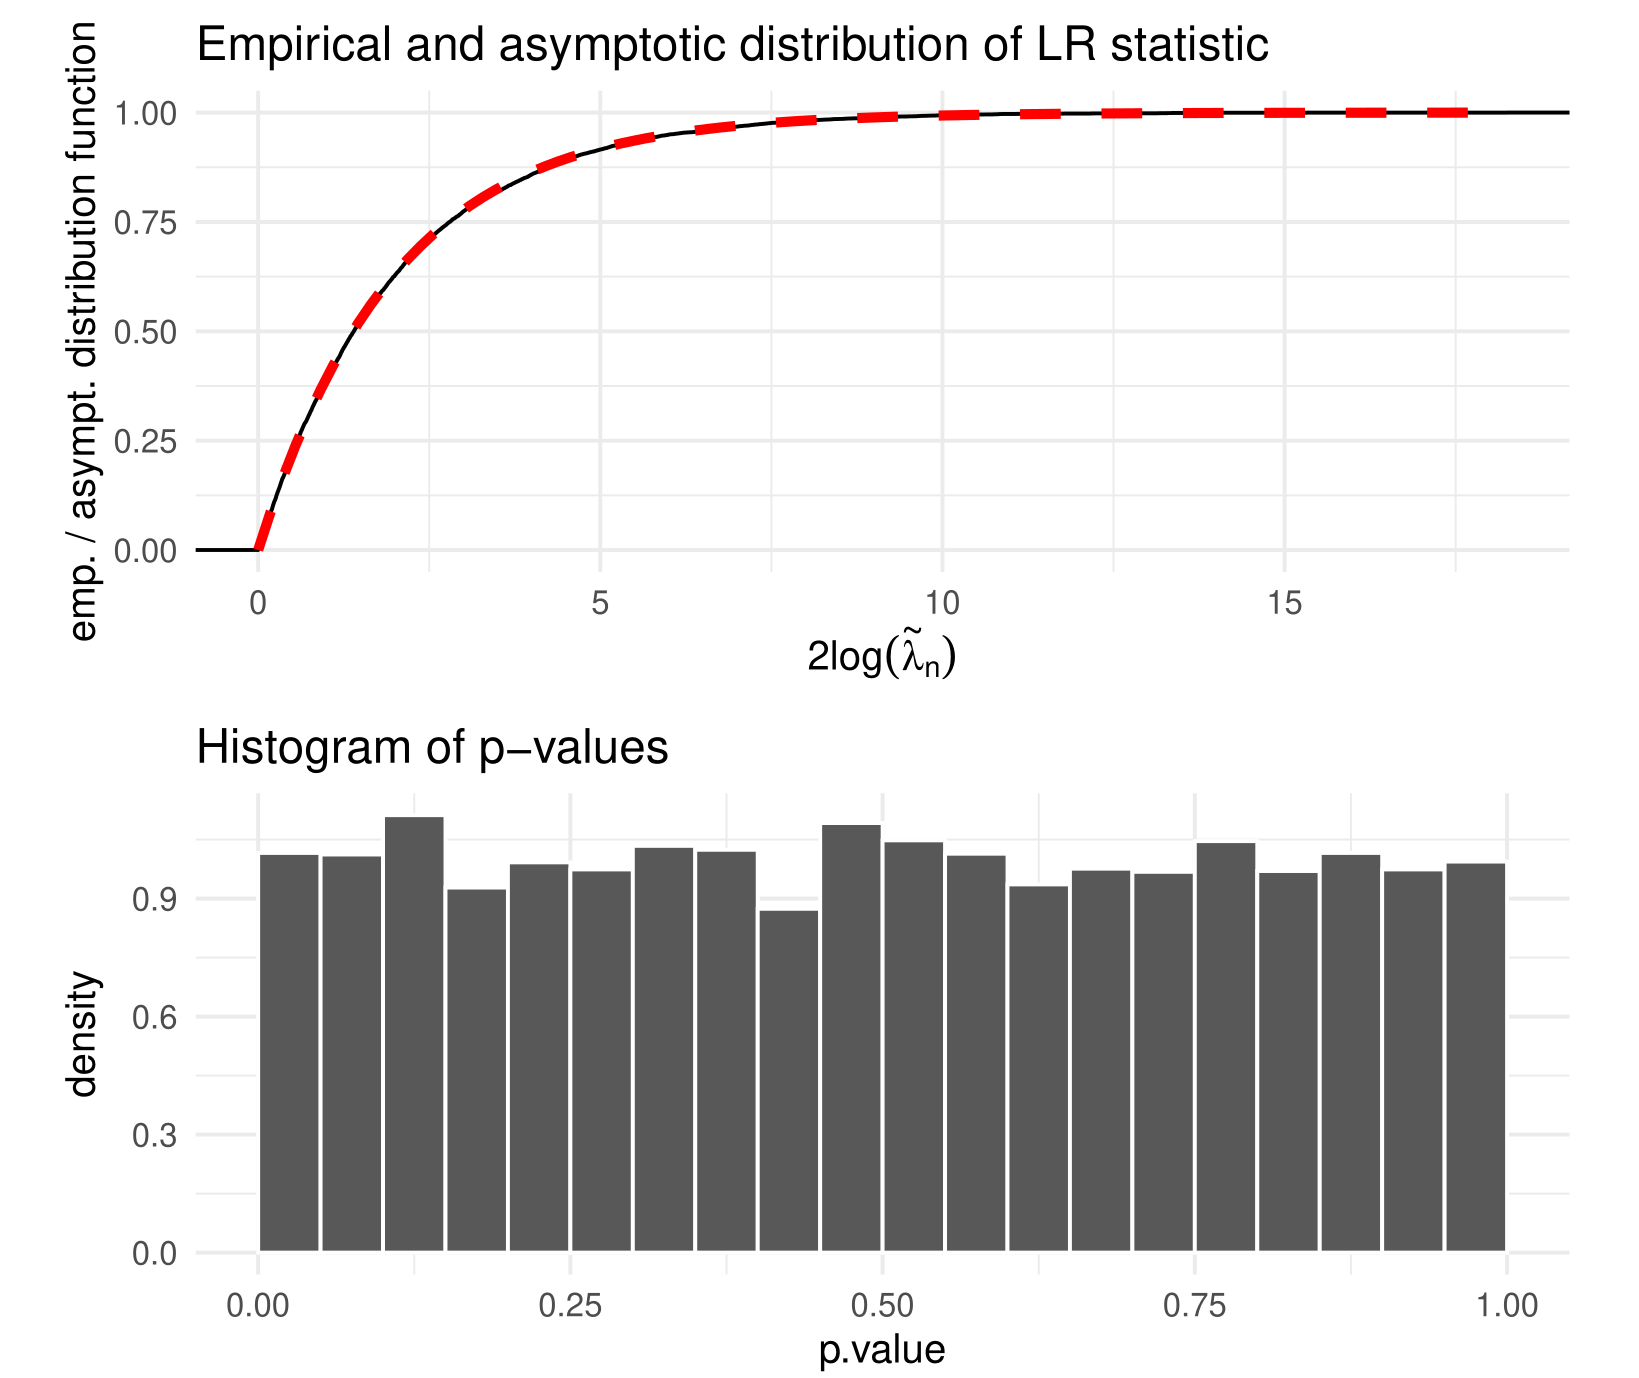
\includegraphics[width=0.8\textwidth]{img/pvalue}
    \caption{}
    \label{fig:pvalue}
\end{figure}

\begin{remark}
Under $H_0$, the simulated $p$-values are approximately uniformly distributed on $[0,1]$, confirming that the likelihood ratio test is well calibrated even for moderate sample sizes such as $n=100$.
\end{remark}

\subsubsection{Interpretation and Use in Regression Models}

\begin{note}
Likelihood ratio tests are routinely implemented in statistical software. In regression settings, such as logistic regression, they are commonly used to compare nested models by testing whether a subset of regression coefficients is equal to zero.
\end{note}

\begin{ex}[Likelihood ratio tests in logistic regression]
Suppose a categorical variable such as age group is encoded using two dummy variables. Testing whether age has an effect corresponds to testing whether both associated regression coefficients are zero. This hypothesis is naturally assessed using a likelihood ratio test with a chi-square reference distribution, where the degrees of freedom equal the number of constrained parameters.
\end{ex}

\subsection{Fixed Alternatives}

\begin{theo}[Fixed Alternatives]\label{thm:fixed-alternatives}
Suppose \(H_0\) is false and \(X_1,X_2,\dots\) are i.i.d.\ with distribution \(\mathsf{P}_{\bs{\theta}}\), where \(\bs{\theta} \neq \bs{\theta}_0\).
Assume that regularity conditions A0--A4 hold at both \(\bs{\theta}\) and \(\bs{\theta}_0\).
Then, as \(n \to \infty\),
\begin{equation}\label{eq:lr-fixed}
\frac{1}{n} \, 2 \log \widetilde{\lambda}_n
\stackrel{p}{\longrightarrow}
2 \, \mathsf{KL}(\mathsf{P}_{\bs{\theta}} \mid \mathsf{P}_{\bs{\theta}_0})
\equiv
2 \, \mathsf{E}_{X \sim \mathsf{P}_{\bs{\theta}}}
\left[
\log \frac{p_{\bs{\theta}}(X)}{p_{\bs{\theta}_0}(X)}
\right]
> 0 ,
\end{equation}
and
\begin{equation}\label{eq:wald-fixed}
\frac{1}{n} \widetilde{W}_n
\stackrel{p}{\longrightarrow}
(\bs{\theta} - \bs{\theta}_0)^{\top}
\mathsf{I}(\bs{\theta})
(\bs{\theta} - \bs{\theta}_0)
> 0 .
\end{equation}

If in addition:

\[
    A5: \quad \quad \quad 
\mathsf{E}_{\theta}
\big[
\lvert \dot{\ell}_j(\theta_0 \mid X_1) \rvert
\big]
< \infty \quad 
\forall j = 1,\dots,d,
\]
then

\begin{equation}\label{eq:rao-fixed}
\frac{1}{n} R_n
\xrightarrow{p}
\mathsf{E}_{\theta}
\big[
\dot{\ell}(\theta_0 \mid X_1)
\big]^{\top}
\mathsf{I}(\theta_0)^{-1}
\mathsf{E}_{\theta}
\big[
\dot{\ell}(\theta_0 \mid X_1)
\big]
> 0 .
\end{equation}
\end{theo}

\begin{remark}
The ordering in the Kullback--Leibler divergence in \eqref{eq:lr-fixed} is essential.
Since the data are generated from \(\mathsf{P}_{\theta}\), expectations are taken with respect to \(\mathsf{P}_{\theta}\), and the divergence must be \(\mathsf{KL}(\mathsf{P}_{\theta} \mid \mathsf{P}_{\theta_0})\).
If \(\theta \neq \theta_0\), this quantity is strictly positive.
\end{remark}

\begin{remark}
Equations \eqref{eq:lr-fixed} and \eqref{eq:wald-fixed} show that, under fixed alternatives,
the likelihood ratio and Wald statistics grow linearly with \(n\), up to stochastic fluctuations.
In contrast, under the null hypothesis, these statistics have non-degenerate stochastic limits.
\end{remark}


\begin{proof}
\textbf{Likelihood ratio statistic.}
Write
\begin{equation*}\label{eq:lr-decomp}
\frac{2}{n} \log \widetilde{\lambda}_n
=
\frac{2}{n}
\big[
\ell(\widetilde{\bs{\theta}}_n) - \ell(\bs{\theta})
\big]
+
\frac{2}{n}
\big[
\ell(\bs{\theta}) - \ell(\bs{\theta}_0)
\big].
\end{equation*}
Since
\(2[\ell(\widetilde{\bs{\theta}}_n) - \ell(\bs{\theta})] \xrightarrow{d} \chi^2_d\),
we have
\[
\frac{2}{n}
\big[
\ell(\widetilde{\bs{\theta}}_n) - \ell(\bs{\theta})
\big]
= o_p(1).
\]
Moreover,
\[
\frac{2}{n}
\big[
\ell(\bs{\theta}) - \ell(\bs{\theta}_0)
\big]
=
2 \cdot \frac{1}{n}
\sum_{i=1}^n
\log \frac{p_{\bs{\theta}}(X_i)}{p_{\bs{\theta}_0}(X_i)}
\xrightarrow{p}
2 \, \mathsf{KL}(\mathsf{P}_{\bs{\theta}} \mid \mathsf{P}_{\bs{\theta}_0}),
\]
by the law of large numbers, proving \eqref{eq:lr-fixed}.

\medskip

\textbf{Wald statistic.}
By \autoref{thm:cmt},
\[
\frac{1}{n} \widetilde{W}_n
=
(\widetilde{\bs{\theta}}_n - \theta_0)^{\top}
\widehat{\mathsf{I}}(\widetilde{\bs{\theta}}_n)
(\widetilde{\bs{\theta}}_n - \theta_0)
\xrightarrow{p}
(\bs{\theta} - \theta_0)^{\top}
\mathsf{I}(\bs{\theta})
(\bs{\theta} - \theta_0),
\]
establishing \eqref{eq:wald-fixed}.

\medskip

\textbf{Rao's score statistic.}
We may write
\[
\frac{1}{n} R_n
=
\left(
\frac{1}{n} \dot{\ell}(\bs{\theta}_0)
\right)^{\top}
\mathsf{I}(\bs{\theta}_0)^{-1}
\left(
\frac{1}{n} \dot{\ell}(\bs{\theta}_0)
\right).
\]
Thus it suffices to show
\[
\frac{1}{n} \dot{\ell}(\bs{\theta}_0)
\stackrel{p}{\longrightarrow}
\mathsf{E}_{\bs{\theta}}
\big[
\dot{\ell}(\bs{\theta}_0 \mid X_1)
\big].
\]
By assumption A5, the expectation is finite, and the law of large numbers applies.
This yields \eqref{eq:rao-fixed}.
\end{proof}

\begin{note}[Interpretation]\label{note:interpretation-fixed}
Under fixed alternatives, all three classical test statistics
(likelihood ratio, Wald, and Rao)
diverge at rate \(n\).
In contrast, under the null hypothesis, they converge in distribution to non-degenerate
\(\chi^2\) limits.
\end{note}

\section{Consistency}

\begin{corollary}[Consistency of Likelihood-Based Tests]\label{cor:consistency}
Under the assumptions of \autoref{thm:fixed-alternatives}, the likelihood ratio and Wald tests are consistent.
That is, if \(\bs{\theta} \neq \theta_0\),
\begin{equation*}\label{eq:consistency-lr-wald}
\mathsf{P}_{\bs{\theta}}(\text{rejection of } H_0) \longrightarrow 1
\quad \text{as } n \to \infty .
\end{equation*}
The same conclusion holds for Rao's score test provided
\(\mathsf{E}_{\bs{\theta}}[\dot{\ell}(\theta_0 \mid X_1)] \neq 0\), in which case
\begin{equation*}\label{eq:rao-positive}
\mathsf{E}_{\bs{\theta}}
\big[
\dot{\ell}(\bs{\theta}_0 \mid X_1)
\big]^{\top}
\mathsf{I}(\bs{\theta}_0)^{-1}
\mathsf{E}_{\bs{\theta}}
\big[
\dot{\ell}(\bs{\theta}_0 \mid X_1)
\big]
> 0 .
\end{equation*}
\end{corollary}

\begin{proof}
The argument is analogous to the proof of \autoref{thm:fixed-alternatives}.
Under fixed alternatives, the test statistics divided by \(n\) converge in probability to strictly positive constants,
whereas under the null hypothesis they have non-degenerate stochastic limits.
Hence, with a fixed rejection threshold, the probability of rejection converges to one.
\end{proof}

\begin{remark}[Why consistency holds]\label{rem:why-consistent}
Under \(H_0\), the likelihood ratio, Wald, and Rao statistics fluctuate in a bounded stochastic range
(e.g.\ they converge in distribution to a \(\chi^2\) law).
If \(H_0\) is false, each statistic behaves like a positive constant times \(n\), up to random noise.
Since the rejection threshold is fixed, the statistic eventually exceeds it with probability tending to one.
\end{remark}

\begin{ex}[Geometric intuition]\label{ex:geometric}
    \leavevmode
\begin{itemize}[]
\item The likelihood ratio statistic measures separation between \(\mathsf{P}_{\bs{\theta}}\) and \(\mathsf{P}_{\bs{\theta}_0}\)
via the Kullback--Leibler divergence.
\item The Wald statistic measures the squared Mahalanobis distance
\((\bs{\theta} - \bs{\theta}_0)^{\top} \mathsf{I}(\bs{\theta}) (\bs{\theta} - \bs{\theta}_0)\).
\item Both quantities are strictly positive when \(\bs{\theta} \neq \bs{\theta}_0\).
\end{itemize}
\end{ex}

\subsubsection{Local Alternatives}

\begin{definition}[Local Alternatives]\label{def:local-alt}
Let \(t \in \mathbb{R}^d\).
A sequence of local alternatives is defined by
\[
\bs{\theta}_n = \bs{\theta}_0 + \frac{\bs{t}}{\sqrt{n}},
\]
and the corresponding distributions
\(\mathsf{P}_{\bs{\theta}_n}\).
\end{definition}


\begin{theo}[Asymptotic Distribution of the MLE under Local Alternatives]\label{thm:mle-local}
Assume that regularity conditions A0--A4 hold at \(\bs{\theta}_0\).
Then, under \(\mathsf{P}_{\bs{\theta}_n}\),
\begin{equation*}\label{eq:mle-local}
\sqrt{n}(\widetilde{\bs{\theta}}_n - \bs{\theta}_0)
\stackrel{d}{\longrightarrow}
\mathcal{N}_d\big(
\bs{t}, \mathsf{I}(\bs{\theta}_0)^{-1}
\big).
\end{equation*}
\end{theo}

\begin{theo}[Non-Central Limit of Test Statistics]\label{thm:noncentral}
Under the local alternatives of \autoref{def:local-alt},
the likelihood ratio, Wald, and Rao statistics converge in distribution to
a non-central chi-square law,
\begin{equation}\label{eq:noncentral-chi}
\chi^2_d\!\left(
\bs{t}^{\top} \mathsf{I}(\theta_0) \bs{t}
\right),
\end{equation}
with non-centrality parameter
\(\bs{t}^{\top} \mathsf{I}(\theta_0) \bs{t}\).
\end{theo}

\begin{remark}[Interpretation]\label{rem:local-int}
Local alternatives make the testing problem harder as \(n\) increases:
while the sample size grows, the parameter \(\theta_n\) approaches the null at rate \(1/\sqrt{n}\).
The non-centrality parameter in \eqref{eq:noncentral-chi} quantifies how far the alternative is from the null
in the metric induced by the Fisher information.
\end{remark}

\begin{note}[Power and sample size planning]\label{note:power}
The non-central chi-square limits in \autoref{thm:noncentral} provide a basis for
power calculations and sample size planning.
Given a model (e.g.\ logistic regression), one can choose \(\bs{t}\) to represent
a scientifically meaningful effect size and compute the resulting power.
\end{note}

\begin{remark}[Further reading]\label{rem:reading}
A systematic treatment of local alternatives relies on contiguity theory,
developed by Lucien Le Cam.
A key result is Le Cam's third lemma, which yields joint convergence results
for likelihood ratios and test statistics.
See Wellner (2018, Chapter~4) and van der Vaart (1998, Chapter~16) for details.
\end{remark}

\section{Composite Null Hypotheses}

\subsection{Test Statistics}

Often one is interested in testing hypotheses that concern only a subset of the parameters.
Let the parameter vector be partitioned as
\begin{equation*}\label{eq:theta-partition}
\bs{\theta} =
\begin{pmatrix}
\bs{\theta}_1 \\
\bs{\theta}_2
\end{pmatrix}
\in \mathbb{R}^m \times \mathbb{R}^{d-m},
\end{equation*}
where \(\bs{\theta}_1\) is the parameter of primary interest and \(\bs{\theta}_2\) is a nuisance parameter.
We consider the composite null hypothesis
\begin{equation}\label{eq:composite-null}
H_0 : \bs{\theta}_1 = \bs{\theta}_{10}
\quad \text{vs.} \quad
H_1 : \bs{\theta}_1 \neq \bs{\theta}_{10},
\end{equation}
where \(\bs{\theta}_{10}\) is a specified value, while \(\bs{\theta}_2\) remains unrestricted.

\begin{remark}
The null hypothesis \eqref{eq:composite-null} is composite because it contains many parameter values:
all vectors \(\bs{\theta} = (\bs{\theta}_{10}, \bs{\theta}_2)\) with arbitrary \(\bs{\theta}_2\).
A classical example is testing whether the mean of a Gaussian distribution equals a fixed value
when the variance is unknown.
\end{remark}

\subsubsection{Likelihood Ratio Statistic}

\begin{definition}[Likelihood Ratio Statistic]\label{def:lr-composite}
Let \(\hat{\bs{\theta}}_n = (\hat{\bs{\theta}}_{n1}, \hat{\bs{\theta}}_{n2})\) denote the unrestricted MLE in
\(\{\mathsf{P}_{\bs{\theta}} : \bs{\theta} \in \Theta\}\),
and let
\(\hat{\bs{\theta}}_n^0 = (\bs{\theta}_{10}, \hat{\bs{\theta}}_{n2}^0)\)
be the MLE under the constraint \(\bs{\theta}_1 = \bs{\theta}_{10}\).
The likelihood ratio statistic is defined as
\begin{equation*}\label{eq:lr-composite}
2 \log \lambda_n,
\qquad
\lambda_n
:=
\frac{\sup_{\bs{\theta} \in \Theta} L(\bs{\theta})}
{\sup_{\bs{\theta} \in \Theta,\, \bs{\theta}_1 = \bs{\theta}_{10}} L(\bs{\theta})}
=
\frac{L(\hat{\bs{\theta}}_n)}{L(\hat{\bs{\theta}}_n^0)}.
\end{equation*}
\end{definition}

\begin{remark}
The numerator optimizes the likelihood over the full parameter space,
while the denominator optimizes only over the null model.
Hence \(\lambda_n \geq 1\) and \(2 \log \lambda_n \geq 0\).
Large values provide evidence against \(H_0\).
\end{remark}

\subsubsection{Rao's Score Statistic}

\begin{definition}[Rao's Score Statistic]\label{def:rao-composite}
Let \(\hat{\bs{\theta}}_n^0\) be the MLE under the null hypothesis.
Rao's score statistic for the composite null is
\begin{equation}\label{eq:rao-composite}
R_n
=
\frac{1}{n}
\dot{\ell}(\hat{\bs{\theta}}_n^0)^{\top}
\widehat{\mathsf{I}}(\hat{\bs{\theta}}_n^0)^{-1}
\dot{\ell}(\hat{\bs{\theta}}_n^0).
\end{equation}
\end{definition}

\begin{remark}
The statistic \eqref{eq:rao-composite} measures whether the MLE under the null
is close to satisfying the first-order optimality conditions of the unrestricted likelihood.
Some score components vanish by construction, while others need not;
their joint magnitude is assessed through the quadratic form.
\end{remark}

\subsubsection{Wald Statistic}

\begin{definition}[Partitioned Fisher Information]\label{def:partition-info}
Partition the Fisher information matrix as
\begin{equation*}\label{eq:info-partition}
\mathsf{I}(\bs{\theta})
=
\begin{pmatrix}
\mathsf{I}_{11}(\bs{\theta}) & \mathsf{I}_{12}(\bs{\theta}) \\
\mathsf{I}_{21}(\bs{\theta}) & \mathsf{I}_{22}(\bs{\theta})
\end{pmatrix}.
\end{equation*}
The Schur complement of \(\mathsf{I}_{22}(\bs{\theta})\) is
\begin{equation*}\label{eq:schur}
\mathsf{I}_{11.2}(\bs{\theta})
=
\mathsf{I}_{11}(\bs{\theta})
-
\mathsf{I}_{12}(\bs{\theta})
\mathsf{I}_{22}(\bs{\theta})^{-1}
\mathsf{I}_{21}(\bs{\theta}),
\end{equation*}
and satisfies
\((\mathsf{I}(\bs{\theta})^{-1})_{11} = \mathsf{I}_{11.2}(\bs{\theta})^{-1}\).
\end{definition}

\begin{definition}[Wald Statistic]\label{def:wald-composite}
Let \(\hat{\bs{\theta}}_{n1}\) be the first \(m\) components of the unrestricted MLE \(\hat{\bs{\theta}}_n\).
The Wald statistic for testing \eqref{eq:composite-null} is
\begin{equation*}\label{eq:wald-composite}
W_n
=
n
(\hat{\bs{\theta}}_{n1} - \bs{\theta}_{10})^{\top}
\widehat{\mathsf{I}}_{11.2}(\hat{\bs{\theta}}_n)
(\hat{\bs{\theta}}_{n1} - \bs{\theta}_{10}).
\end{equation*}
\end{definition}

\begin{remark}
The Wald test compares the unrestricted estimate of \(\bs{\theta}_1\)
to its hypothesized value \(\bs{\theta}_{10}\),
while appropriately accounting for nuisance parameters through the
Schur complement \(\widehat{\mathsf{I}}_{11.2}(\hat{\bs{\theta}}_n)\).
\end{remark}

\begin{ex}[Gaussian Mean with Unknown Variance]\label{ex:gaussian-composite}
Let \(X_1,\dots,X_n \sim \mathcal{N}(\mu,\sigma^2)\).
To test \(H_0 : \mu = 7\) with unknown \(\sigma^2\),
\begin{itemize}[]
\item \(\bs{\theta}_1 = \mu\), \(\bs{\theta}_2 = \sigma^2\),
\item the likelihood ratio compares the unrestricted MLE
\((\hat{\mu},\hat{\sigma}^2)\) to the constrained MLE \((7,\hat{\sigma}_0^2)\),
\item the Wald statistic assesses whether \(\hat{\mu}\) is close to \(7\),
accounting for uncertainty in \(\hat{\sigma}^2\).
\end{itemize}
\end{ex}

\begin{note}[Practical considerations]\label{note:computation}
    \leavevmode
\begin{itemize}[]
\item The likelihood ratio test requires two optimizations:
one unrestricted and one under the null.
\item Rao's test requires only optimization under the null.
\item The Wald test uses the unrestricted MLE and an estimate of the
partitioned Fisher information.
\end{itemize}
\end{note}

\subsection{Chi-Square Limits for Composite Null Hypotheses}

As before, assume that the estimator $\tilde{\bs{\theta}}_n$ is a consistent solution of the likelihood equations for the model
$\{\mathsf{P}_{\bs{\theta}} : \bs{\theta} \in \Theta\}$.

Similarly, assume that $\tilde{\bs{\theta}}_n^0$ is a consistent solution of the likelihood equations for the null model with
$\bs{\theta}_1 = \bs{\theta}_{10}$.

We write $\tilde{\lambda}_n$, $\widetilde{W}_n$, and $\widetilde{R}_n$ to indicate the use of $\tilde{\bs{\theta}}_n$ and
$\tilde{\bs{\theta}}_n^0$ instead of $\hat{\bs{\theta}}_n$ and $\hat{\bs{\theta}}_n^0$.

\begin{theo}[Null distribution / Wilks' Theorem]\label{thm:wilks}
Suppose assumptions A0--A4 hold at the true parameter
$\bs{\theta}_0 = (\bs{\theta}_{01}, \bs{\theta}_{02})^\top \in \mathbb{R}^m \times \mathbb{R}^{d-m}$,
and assume that $\bs{\theta}_{01} = \bs{\theta}_{10}$, so that $H_0$ is true. Then
\begin{equation*}
\left.
\begin{array}{l}
2 \log \tilde{\lambda}_n \\
\widetilde{W}_n \\
\widetilde{R}_n
\end{array}
\right\}
\xrightarrow{d} \chi^2_m .
\end{equation*}
\end{theo}

\begin{remark}
The degrees of freedom $m$ equal the number of imposed constraints, or equivalently the difference between the dimension
of the alternative model ($d$) and the dimension of the null model ($d-m$).
\end{remark}

\begin{proof}[]
\subsubsection*{Wald Statistic}

Define
\begin{equation*}
\bs{D}
=
\begin{pmatrix}
\bs{D}_1 \\
\bs{D}_2
\end{pmatrix}
:=
\mathbf{I}(\bs{\theta}_0)^{-1} \bs{Z},
\qquad
\bs{Z} \sim \mathcal{N}_d(\bs{0}, \mathbf{I}(\bs{\theta}_0)).
\end{equation*}
Then $\bs{D} \sim \mathcal{N}_d(\bs{0}, \mathbf{I}(\bs{\theta}_0)^{-1})$ and
\begin{equation*}
\sqrt{n}(\tilde{\bs{\theta}}_{n1} - \bs{\theta}_{10})
\xrightarrow{d}
\bs{D}_1
\sim
\mathcal{N}_m(\bs{0}, (\mathbf{I}(\bs{\theta}_0)^{-1})_{11})
=
\mathcal{N}_m(\bs{0}, \mathbf{I}_{11.2}(\bs{\theta}_0)^{-1}).
\end{equation*}

Since $\hat{\mathbf{I}}(\tilde{\bs{\theta}}_n) \xrightarrow{p} \mathbf{I}(\bs{\theta}_0)$, we also have
$\hat{\mathbf{I}}_{11.2}(\tilde{\bs{\theta}}_n) \xrightarrow{p} \mathbf{I}_{11.2}(\bs{\theta}_0)$.
Therefore,
\begin{equation*}
\widetilde{W}_n
\xrightarrow{d}
\bs{D}_1^\top \mathbf{I}_{11.2}(\bs{\theta}_0)\bs{D}_1
\sim
\chi^2_m .
\end{equation*}

\begin{note}
The Schur complement $\mathbf{I}_{11.2}$ represents the Fisher information about $\bs{\theta}_1$ in the presence of the nuisance
parameter $\bs{\theta}_2$. It also corresponds to the inverse asymptotic covariance matrix of $\sqrt{n}(\tilde{\bs{\theta}}_{n1}-\bs{\theta}_{10})$.
\end{note}

\subsubsection*{Rao (Score) Statistic}

Partition the score function as
\begin{equation*}
\dot{\ell}(\tilde{\bs{\theta}}_n^0)
=
\begin{pmatrix}
\dot{\ell}_1(\tilde{\bs{\theta}}_n^0) \\
\dot{\ell}_2(\tilde{\bs{\theta}}_n^0)
\end{pmatrix}.
\end{equation*}
Since $\tilde{\bs{\theta}}_n^0$ maximizes the likelihood under $H_0$, we have
$\dot{\ell}_2(\tilde{\bs{\theta}}_n^0)=\bs{0}$.

A Taylor expansion around $\bs{\theta}_0$ yields
\begin{equation*}
\frac{1}{\sqrt{n}}\dot{\ell}_1(\tilde{\bs{\theta}}_n^0)
=
\frac{1}{\sqrt{n}}\dot{\ell}_1(\bs{\theta}_0)
-
\mathbf{I}_{12}(\bs{\theta}_0)\sqrt{n}(\tilde{\bs{\theta}}_{n2}^0-\bs{\theta}_{02})
+ o_p(1).
\end{equation*}
Using asymptotic linearity of the MLE under the null model,
\begin{equation*}
\sqrt{n}(\tilde{\bs{\theta}}_{n2}^0-\bs{\theta}_{02})
=
\mathbf{I}_{22}(\bs{\theta}_0)^{-1}
\frac{1}{\sqrt{n}}\dot{\ell}_2(\bs{\theta}_0)
+ o_p(1).
\end{equation*}
Hence,
\begin{equation*}
\frac{1}{\sqrt{n}}\dot{\ell}_1(\tilde{\bs{\theta}}_n^0)
\xrightarrow{d}
\bs{Z}_1 - \mathbf{I}_{12}(\bs{\theta}_0)\mathbf{I}_{22}(\bs{\theta}_0)^{-1}\bs{Z}_2,
\end{equation*}
where $(\bs{Z}_1^\top,\bs{Z}_2^\top)^\top \sim \mathcal{N}_d(\bs{0},\mathbf{I}(\bs{\theta}_0))$.

Now, we have that
\begin{equation*}
\bs{Z}_1 - \mathbf{I}_{12}(\bs{\theta}_0)\mathbf{I}_{22}(\bs{\theta}_0)^{-1}\bs{Z}_2
\sim
\mathcal{N}_m(\bs{0},\mathbf{I}_{11.2}(\bs{\theta}_0)).
\end{equation*}

Therefore,
\begin{equation*}
\widetilde{R}_n
=
\frac{1}{n}
\dot{\ell}_1(\tilde{\bs{\theta}}_n^0)^\top
\hat{\mathbf{I}}_{11.2}(\tilde{\bs{\theta}}_n^0)^{-1}
\dot{\ell}_1(\tilde{\bs{\theta}}_n^0)
\xrightarrow{d}
\chi^2_m .
\end{equation*}

\begin{remark}
The Rao statistic measures whether the MLE under the null is already close to satisfying the full
first-order optimality conditions of the unrestricted model.
\end{remark}

\subsubsection*{Likelihood Ratio Statistic}

Write
\begin{equation*}
2\log\tilde{\lambda}_n
=
2\big(\ell(\tilde{\bs{\theta}}_n)-\ell(\bs{\theta}_0)\big)
-
2\big(\ell(\tilde{\bs{\theta}}_n^0)-\ell(\bs{\theta}_0)\big).
\end{equation*}
By standard likelihood theory,
\begin{align*}
2\big(\ell(\tilde{\bs{\theta}}_n)-\ell(\bs{\theta}_0)\big)
&\xrightarrow{d}
\bs{Z}^\top \mathbf{I}(\bs{\theta}_0)^{-1}\bs{Z},\\
2\big(\ell(\tilde{\bs{\theta}}_n^0)-\ell(\bs{\theta}_0)\big)
&\xrightarrow{d}
\bs{Z}_2^\top \mathbf{I}_{22}(\bs{\theta}_0)^{-1}\bs{Z}_2,
\end{align*}
jointly. Hence,
\begin{equation*}
2\log\tilde{\lambda}_n
\xrightarrow{d}
\bs{D}_1^\top \mathbf{I}_{11.2}(\bs{\theta}_0)\bs{D}_1
\sim
\chi^2_m .
\end{equation*}
\end{proof}

\begin{remark}
All three statistics are asymptotically equivalent. Their differences are of order $o_p(1)$
and vanish asymptotically.
\end{remark}

\begin{ex}[Simulation Illustration]
For a Gamma$(5,2)$ model with sample size $n=150$, simulate $10{,}000$ datasets and compute
$2\log\tilde{\lambda}_n$ under a composite null hypothesis. The empirical distribution function
closely matches the $\chi^2_m$ distribution, and the corresponding $p$-value distribution
is approximately uniform, confirming correct calibration.
\end{ex}



\begin{ex}[Likelihood ratio test for Gamma model]
We compute the \emph{p}-value for testing
\[
H_0 : \alpha = 4
\]
based on a sample from the $\mathrm{Gamma}(5,2)$ distribution.

Under $H_0$, we optimize the negative log-likelihood with respect to $\beta$ while fixing
$\alpha=\alpha_0$.
\end{ex}

\begin{definition}[Negative log-likelihood under the null]
Let $\alpha_0>0$ be fixed. The negative log-likelihood under $H_0$ is given by
\begin{equation*}
\ell_0(\beta; \bs{x}, \alpha_0)
=
-\sum_{i=1}^n \log f_{\alpha_0,\beta}(x_i),
\end{equation*}
where $f_{\alpha,\beta}$ denotes the Gamma density with shape $\alpha$ and rate $\beta$.
\end{definition}

\begin{minted}{r}
negloglik0 = function(b, data, a0){
    a = a0
    n = length(data)
    return(
        -sum(dgamma(data, shape = a, rate = b, log = TRUE))
    )
}
\end{minted}

\paragraph{Data generation}%
We generate a sample of size $n=150$ from a $\mathrm{Gamma}(5,2)$ distribution.

\begin{minted}{r}
set.seed(22)
n <- 150
x <- rgamma(n, shape = 5, rate = 2)
\end{minted}

\paragraph{Optimization under null and alternative}%

We optimize the negative log-likelihood under $H_0$ and under the unrestricted model.

\begin{minted}{r}
opt0 <- optimize(negloglik0, c(0, 100), data = x, a0 = 4)
opt1 <- optim(c(1,1), negloglik, data = x)
\end{minted}

\begin{definition}[Likelihood ratio statistic]
The likelihood ratio statistic is defined as
\begin{equation*}
\Lambda_n
=
2\bigl(\ell(\hat{\alpha},\hat{\beta}) - \ell(\alpha_0,\hat{\beta}_0)\bigr),
\end{equation*}
where $(\hat{\alpha},\hat{\beta})$ denotes the unrestricted MLE and $\hat{\beta}_0$ the MLE under $H_0$.
\end{definition}

\begin{minted}{r}
lambda <- 2*(-opt1$value - (-opt0$objective))
lambda
\end{minted}

This yields $\Lambda_n \approx 6.99$.

\myparagraph{\(p\)--value computation}%

Under regularity conditions, $\Lambda_n \xrightarrow{d} \chi^2_1$ since one restriction is imposed.

\begin{minted}{r}
p.value <- 1 - pchisq(lambda, df = 1)
p.value
\end{minted}

The resulting $p$-value is approximately $0.008$, indicating strong evidence against $H_0$.

\begin{remark}
Intuitively, the likelihood ratio compares how much more likely the observed data are under the
best-fitting Gamma distribution compared to the Gamma distribution with fixed shape $\alpha=4$.
Here, the unrestricted model is about seven times more likely in terms of density.
\end{remark}

\begin{ex}[Null distribution of LR statistic and \(p\)--value]
\end{ex}
    \paragraph{Simulation under the null}%
    
We now investigate the null distribution of the likelihood ratio statistic and the corresponding
$p$-values for testing
\[
H_0 : \alpha = 5
\]
when the data are generated from a $\mathrm{Gamma}(5,2)$ distribution.

\begin{definition}[Composite likelihood ratio test function]
The following function computes the likelihood ratio statistic and $p$-value, including optimization
under the restricted model.
\end{definition}

\begin{minted}{r}
lr_test_gamma_comp <- function(
    alpha = 1, beta = 1, n = 100, alpha0 = 1){
    x <- rgamma(n = n, shape = alpha, rate = beta)
    opt0 <- optimize(negloglik0, c(0,100),
                     data = x, a0 = alpha0)
    opt1 <- optim(c(1,1), negloglik, data = x)
    stat <- 2*(-opt1$value - (-opt0$objective))
    pval <- 1 - pchisq(stat, df = 1)
    return(data.frame(stat = stat, pval = pval))
}
\end{minted}

\paragraph{Monte Carlo approximation}%

We repeat the test $10{,}000$ times with sample size $n=150$.

\begin{minted}{r}
set.seed(22)

df <- 1:10000 |>
  purrr::map_df(\(i)
    lr_test_gamma_comp(
      alpha = 5, beta = 2, n = 150, alpha0 = 5
    )
  )
\end{minted}

\begin{remark}
For each simulated dataset, we compute $2\log\Lambda_n$ and the corresponding $p$-value.
This yields an empirical distribution of the test statistic under the null.
\end{remark}

\paragraph{Empirical vs asymptotic distribution}%

The empirical distribution function of the simulated statistics is compared to the
$\chi^2_1$ distribution function.

\begin{minted}{r}
p1 <- ggplot(df, aes(x = stat)) +
    stat_ecdf(geom = "step") +
    geom_function(fun = pchisq, args = list(df = 1))
\end{minted}

\begin{remark}
The empirical distribution function is a step function with many small jumps, but it closely
approximates the $\chi^2_1$ distribution. This confirms the validity of the asymptotic approximation.
\end{remark}

\begin{claim}[Calibration of the test]
If the likelihood ratio test is well calibrated, the distribution of $p$-values under $H_0$
should be uniform on $[0,1]$.
\end{claim}

\begin{remark}
In this simulation, the $p$-value histogram is nearly uniform, indicating excellent calibration
for sample size $n=150$ in the Gamma example.
\end{remark}

\begin{note}
Throughout, the nuisance parameter $\beta$ is optimized out under both the null and alternative.
The test focuses solely on the parameter of interest $\alpha$.
\end{note}
\begin{figure}[htpb]
    \centering
    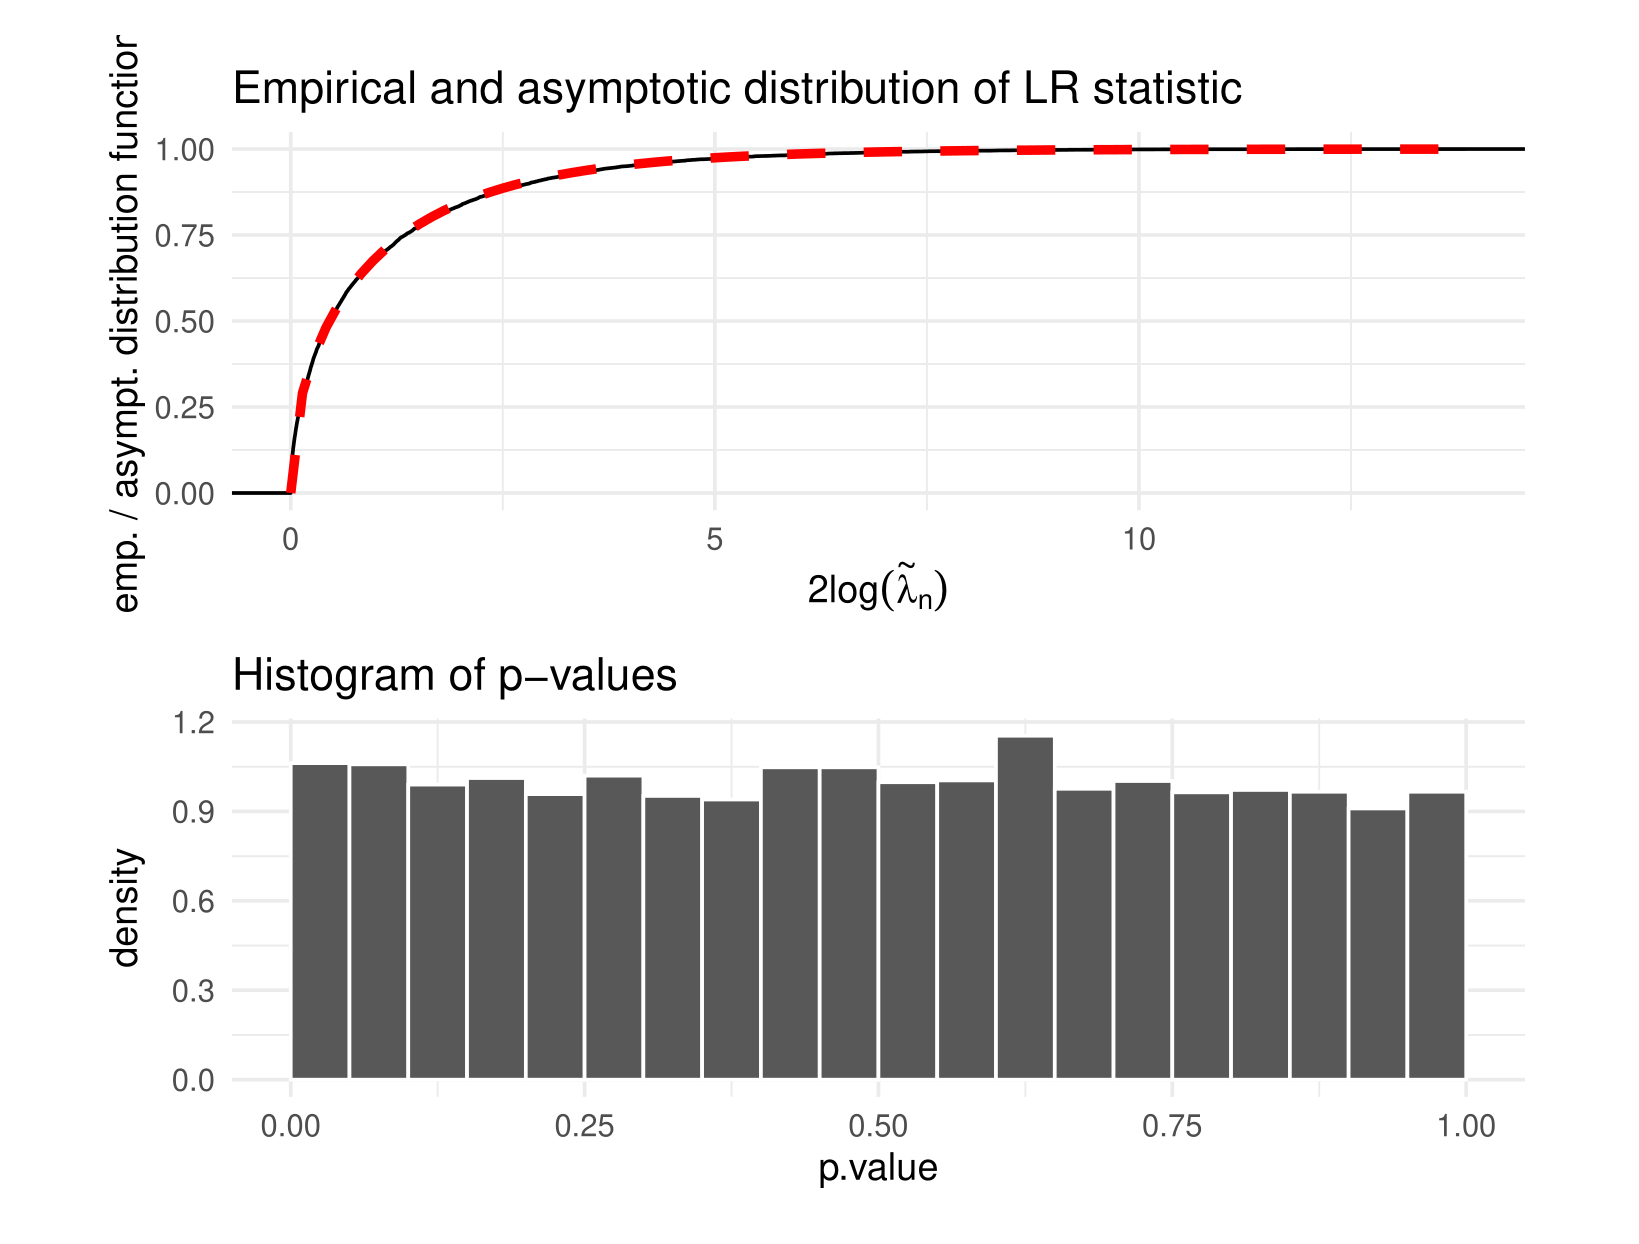
\includegraphics[width=0.8\textwidth]{img/asymptotic}
    \caption{}
    \label{fig:asymptotic}
\end{figure}
